\chapter{Blockchain 2.0}
Durch den Zusammenschluss verschiedenster Vorgängertechnologien gelang es Nakamoto, einen dezentralen Mechanismus zur Verarbeitung von Transaktionen vorzustellen, der mit den bereits bestehenden Institutionen in Punkten wie Sicherheit und Geschwindigkeit konkurrieren kann. Vor allem die Möglichkeit, auf eine dezentrale Art und Weise zu einem gemeinsamen Konsens kommen zu können, macht es zu einer disruptiven Technologie. Als Programmierer jedoch Konzepte, die über das Versenden von Guthaben hinausgehen, entwickeln wollten, wurde dies durch die Einschränkungen des Bitcoin-Protokolls, wie die Block-Dauer von 10 Minuten oder unzureichende Block-Struktur, erschwert. Man kann deshalb von Bitcoin als spezialisierte Blockchain reden, die ihre wenigen Funktionalitäten zufriedenstellend bereitstellt.\\
Im Jahr 2013 veröffentlichte Vitalik Buterin das Whitepaper \cite{buterin_whitepaper_2013}, in dem er Konzepte für eine neue Blockchain namens Ethereum vorstellte. Dabei handelt es sich um den Entwurf für eine Art Welt-Computer, der sich von Bitcoin vor Allem in den folgenden Punkten unterscheidet:
\begin{enumerate}
	\item Es können beliebige Daten auf der Blockchain gespeichert werden
	\item Es kann Code auf der Blockchain hinterlegt und dort ausgeführt werden
	\end{enumerate}
Im Gegensatz zum Bitcoin-Protokoll, welches zwischen den Blöcken nur eine Veränderung des UTXO-Sets aufweist, stellt Ethereum einen globalen State dar, in dem neben den Aufzeichnungen zu den Guthaben der Teilnehmer auch andere beliebige Daten abgespeichert werden können. Damit geht Ethereum über den Einsatz als Geldsystem hinaus.
Über spezielle Adressen erlaubt das Ethereum-Protokoll das hinterlegen von kompilierten Code direkt auf der Blockchain, welcher über Transaktionen getriggert werden und den State modifizieren kann. 
\\
Ethereum übernimmt viele Konzepte, die bereits aus dem Kapitel \emph{Blockchain 1.0} bekannt sind (Keys, Wallets, Mining, etc.). Dieses Kapitel befasst sich mit Neuerungen, die das Ausführen von Smart-Contracts ermöglichen bzw. durch diese ermöglicht werden.
\section{Theoretische Grundlagen von Ethereum}
Im Gegensatz zum Bitcoin-Protokoll, in dem das UTXO-Modell genutzt wird, kommt beim Ethereum-Protokoll ein sogenanntes \emph{Account Based Model} zum Einsatz. Jede Adresse auf der Blockchain hat ein Guthaben, auf das Ether, die native Währung auf Ethereum, hinzugefügt bzw. abgehoben werden kann. Eine passende Analogie für die beiden Kontenmodelle wäre das UTXO-Modell als physikalische Geldbörse, aus der für eine Transaktion einzelne Münzen (UTXO) herausgesucht und konsumiert werden müssen, sowie das Girokonto, dessen Guthaben beliebig augmentiert werden kann. Dies hat zur Folge, dass andere Mechanismen zum Lösen des Double-Spending-Problems geben muss.

\subsection{Transaktionen}
Neben dem Transfer von Guthaben, so wie es bereits von Bitcoin bekannt ist, dienen Transaktionen auf Ethereum dem Zweck, die Ausführung von, auf der Blockchain hinterlegten, Smart-Contracts auszulösen.
Um diese Funktion erfüllen zu können, unterscheidet sich eine Transaktion auf Ethereum zu deren im Bitcoin-Protokoll:
\begin{lstlisting}
	Transaction {
		nonce;
		recipient;
		value;
		data;
		v;
		r;
		s;	
		gas_price;
		gas_limit;
}
\end{lstlisting}
\emph{Nonce} ist ein Zähler, der bei Transaktionen auf Ethereum eine andere Bedeutung hat, als beim Mining. In einer Transaktion gibt er an, wie viele bestätigte Transaktionen, inklusive sich selbst, bereits von jener Adresse gesendet wurden. Dies führt dazu, dass das Netzwerk eine Warteschlange, aus den von einer Adresse gesendeten Transaktionen, bilden kann. Da im Account-Based-Modell keine UTXO konsumiert werden, kann das Netzwerk anhand des Zählers eine Priorisierung der unbestätigten Transaktionen festlegen und, sollte das gesamte Guthaben nicht ausreichen, Transaktionen mit niedrigerer Priorität ablehnen.\\
Der eigentliche Payload einer Transaktion besteht aus \emph{Value} und \emph{Data}, wobei keines dieser Felder zwingend gefüllt sein muss.
Als Value bezeichnet man die Ether, welche bei einer Transaktion gesendet werden können und je nach Art der Empfängeradresse anders verarbeitet werden. Findet die Transaktion zwischen zwei Teilnehmern des Netzwerkes statt, so werden die Ether der Empfängeradresse zugeschrieben. Handelt es sich dagegen um einen Smart-Contract, so wird dessen Guthaben (Ein Smart-Contract hat eine Adresse und kann dementsprechend Ether halten) erhöht und eine, als \emph{payable} gekennzeichnete, Fallback-Funktion ausgeführt. Bei Fehlen einer solchen Funktion wird ein Fehler geworfen und andernfalls der State des Smart-Contracts angepasst.
Die Fallback-Funktion nur dann ausgeführt, wenn das Feld Data des Payloads leer ist. In diesem selektiert man die gewünschten Funktionen und mit welchen Parametern diese ausgeführt werden sollen. Die Felder \emph{v, r ,s} sind für die Authentifizierung nötig, werden hier aber nicht weiter erörtert. Im Endeffekt werden Transaktionen wie bekannt mit dem privaten Schlüssel signiert und andere Teilnehmer des Netzwerkes validieren diese mit dem öffentlichen Schlüssel.\\
\subsubsection{Neues Konzept: Gas}
In seinem Paper \cite{turing_1936} stellte Alan Turing einen Entwurf für eine Maschine vor, die aus einem nahezu unendlich langem Streifen aus Papier und einem Kopf besteht. Der Streifen ist in Bereiche unterteilt, die jeweils ein Zeichen, wie z.B. eine Zahl, enthalten und zwischen denen sich der Kopf bewegen kann. Dieser ist in der Lage, das Zeichen des Bereiches, 'auf dem er sich befindet', zu lesen, zu überschreiben, zu löschen oder auch auf dem Streifen zu verschieben. Die Maschine ermöglicht somit, in Abhängigkeit zu den gegebenen Instruktionen, das Berechnen sowie abspeichern beliebiger Sequenzen von Zeichen auf dem Streifen. Eine solche Maschine wird heutzutage als Turing-Maschine bezeichnet.\\
Im Ethereum-Whitepaper \cite{buterin_whitepaper_2013} wird Ethereum als Blockchain bezeichnet, die eine Programmiersprache verwendet, welche turing-vollständig ist. Michaelson beschreibt in \cite{Michaelson_2020} turing-vollständige Programmiersprachen als solche, die ihre Berechnungen in Form einer Turing-Maschine ausdrücken können. Dafür dürfen sie laut Michaelson weder in ihren genutzten Werten, noch in den darauf ausgeführten Berechnungen beschränkt sein. Konkret heißt das im Fall von Ethereum und der genutzten Programmiersprache, dass beliebig aufwendige Berechnungen, sowie geforderter Speicherbedarf ermöglicht werden müssen.
Auf einem lokalen Computer kann eine endlos laufende Schleife leicht gestoppt werden, aber im Kontext eines dezentralen Systems würde jene Schleife die Stabilität des gesamten Netzwerkes bedrohen und würde sogar als Angriffsmethode für bösartige Akteure dienen können. Im Endeffekt nutzen die Teilnehmer des Netzwerkes Ressourcen aus dem selben Pool, sodass ein Mechanismus nötig ist, um das Verschwenden dieser begrenzten Ressourcen unattraktiv zu machen.\\
Die Anweisungen, welche in einem Smart-Contract hinterlegt sind, werden nach Triggern durch eine Transaktion von der \emph{Ethereum Virtual Machine} interpretiert und ausgeführt. Jede der Anweisungen verbraucht jedoch \emph{Gas}, welches als neues Konzept zur Lösung der genannten Probleme aus Touring-Vollständigkeit eingeführt wurde. So bleibt die Programmiersprache zwar touring-vollständig, die Ressourcen, welche Teilnehmer in Anspruch nehmen können, werden jedoch begrenzt. Dies hat zur Folge, dass die Anzahl an Gas, sowie der Preis in Ether, welchen man bereit ist zu zahlen, in einer Transaktion angegeben werden muss. Miner suchen sich anschließend die Transaktionen heraus, welche für sie attraktiv sind, und fügen sie zu ihrem Block hinzu. Übrig gebliebenes Gas wird in Form von Ether wieder zurückerstattet. Zu einer Transaktion gehören demnach die, für den Versand bestimmten, Ether, sowie jene, welche für den Erwerb von Gas bereitgestellt werden müssen.
\subsection{Ethereum Virtual Machine}
Genau wie im Bitcoin-Protokoll sammeln Miner Transaktionen, validieren diese und versuchen, per Proof-Of-Work einen geeigneten Block zu finden und im Netzwerk zu propagieren. 
Im Gegensatz zu den Transaktionen im Bitcoin-Protokoll lösen die Transaktionen unter Ethereum allerdings die Ausführung von, auf der Blockchain hinterlegten, Smart-Contracts aus. 
Für die Ausführung derer ist die Ethereum Virtual Machine (kurz EVM) zuständig. 
Sie ist eine Virtuelle Maschine, die in  \cite{wood_yellowpaper_2014} als stack-basierte Architektur beschrieben wird. 
Die folgende Abbildung illustriert eine vereinfachte Darstellung ihrer Funktionsweise: 
\begin{figure}[htpb]
	\centering
	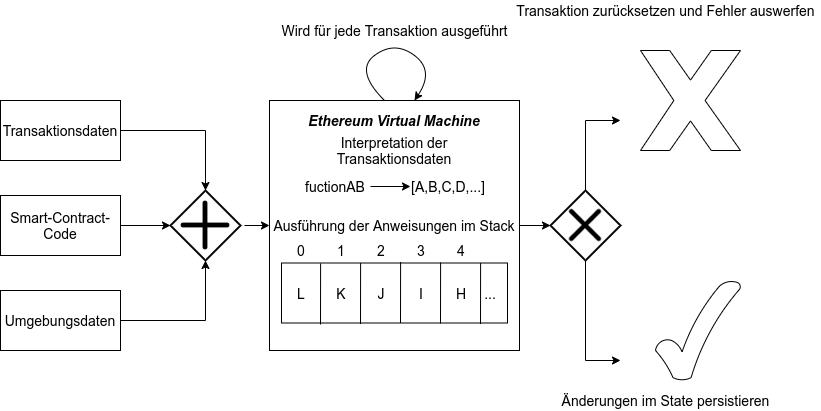
\includegraphics[width=\textwidth]{images/evm_simple.png}
	\caption{Vereinfachung der Ethereum Virtual Machine}
	\label{6braun:fig:evm_simple}
\end{figure}\\
Die EVM erhält als externen Input die Daten für Transaktionen, die sie ausführen muss und wandelt die darin enthaltenen Funktionsaufrufe sowie ihre Parameter in ausführbare Einzeloperationen in Form von Maschinencode um. 
Als zusätzliche Inputs für die Verarbeitung von Transaktionen dienen der Smart-Contract-Code, als auch Umgebungsdaten, wie z.B. die verfügbare Menge an Gas oder das Guthaben der involvierten Adressen. 
Die EVM führt die Anweisungen nach dem LIFO-Prinzip im Kontext der Umgebungsdaten aus und verbraucht für jede Anweisung eine gewisse Menge Gas, die von der Art jener Operation abhängt. Wenn während der Ausführung keine Fehler auftreten, dann wird der State persistiert und mit der nächsten Transaktion fortgefahren. 
Wenn allerdings an einer beliebigen Stelle des Stacks ein Fehler auftritt, sei es beispielsweise durch unzureichendes Gas, wird die gesamte Transaktion zurückgesetzt, da Transaktionen atomar sind und nur in ihrer Gesamtheit ausgeführt werden können. Erst wenn ein valider neuer State erreicht ist, gilt der Block selbst als valide und kann mittels Proof-Of-Work gemined werden. Im Anhang unter \ref{6braun:fig:EVM_full} befindet sich eine umfassende Abbildung aus dem Buch \cite{antanopoulos_2018}.
\subsection{Die Programmiersprache Solidity}
\begin{lstlisting}
	// SPDX-License-Identifier: GPL-3.0
	pragma solidity ^0.8.4;
	contract SimpleAuction {
		address payable public beneficiary;
		uint public auctionEndTime;
		address public highestBidder;
		uint public highestBid;
		
		mapping(address => uint) pendingReturns;
		bool ended;
		event HighestBidIncreased(address bidder, uint amount);
		event AuctionEnded(address winner, uint amount);
		error AuctionAlreadyEnded();
		error BidNotHighEnough(uint highestBid);
		error AuctionNotYetEnded();
		error AuctionEndAlreadyCalled();

		constructor(
		uint _biddingTime,
		address payable _beneficiary
		) {
			beneficiary = _beneficiary;
			auctionEndTime = block.timestamp + _biddingTime;
		}
		
	
		function bid() public payable {
			if (block.timestamp > auctionEndTime)
			revert AuctionAlreadyEnded();
		
			if (msg.value <= highestBid)
			revert BidNotHighEnough(highestBid);
			
			if (highestBid != 0) {
				
				pendingReturns[highestBidder] += highestBid;
			}
			highestBidder = msg.sender;
			highestBid = msg.value;
			emit HighestBidIncreased(msg.sender, msg.value);
		}
		function withdraw() public returns (bool) {
			uint amount = pendingReturns[msg.sender];
			if (amount > 0) {
				pendingReturns[msg.sender] = 0;
				if (!payable(msg.sender).send(amount)) {
					pendingReturns[msg.sender] = amount;
					return false;
				}
			}
			return true;
		}
		
		function auctionEnd() public {
	
			// 1. Conditions
			if (block.timestamp < auctionEndTime)
			revert AuctionNotYetEnded();
			if (ended)
			revert AuctionEndAlreadyCalled();
			// 2. Effects
			ended = true;
			emit AuctionEnded(highestBidder, highestBid);
			
			// 3. Interaction
			beneficiary.transfer(highestBid);
		}
	}
\end{lstlisting}
\section{Weitere Konzepte}
\subsection{DAO}
\subsection{Tokens}
\subsection{DApps}